\documentclass[11pt]{article}
\usepackage[a4paper,margin=2.5cm]{geometry}
\usepackage[T1]{fontenc}
\usepackage{mathptmx}

\usepackage{microtype}
\usepackage{amsmath}
\usepackage{booktabs}
\usepackage{graphicx}
\usepackage{xcolor}
\usepackage[numbers,sort&compress]{natbib}
\usepackage{xurl}
\usepackage[colorlinks=true,linkcolor=blue!50!black,citecolor=blue!50!black,urlcolor=blue!50!black]{hyperref}

\newcommand{\todo}[1]{\textcolor{red}{[TODO: #1]}}

\title{Duplicates, Hospital Shift and Missingness Shortcuts:\\
A Leakage Audit and Leave-One-Hospital-Out Re-evaluation of Machine Learning on the UCI Heart Disease Data}
\author{Muzammal Hussain\\
\small Masmatix Innovations Ltd, Glasgow, United Kingdom\\
\small \texttt{muzammal@masmatixinnovations.co.uk}}
\date{October 2026 \quad (preprint draft)}

\begin{document}
\maketitle

\begin{abstract}
The UCI heart disease data are among the most widely used benchmarks for clinical machine learning, and published accuracies on them often exceed 90\%. We re-evaluate six models, logistic regression, random forest, XGBoost, LightGBM, CatBoost and the tabular foundation model TabPFN, under three protocols. First, a leakage audit of the 1,025-row merged file widely redistributed on Kaggle shows that it contains only 302 distinct records: after a random 80/20 split, 97.1\% of test rows have an exact copy in the training set, and a random forest reaches 0.995 accuracy and 0.999 AUROC, against 0.833 and 0.909 once duplicates are removed. Second, on the original four-hospital data (918 patients after de-duplication), repeated stratified cross-validation places all six models within 0.882--0.907 AUROC, with logistic regression (0.904) level with TabPFN (0.907). Third, leave-one-hospital-out validation reveals a consistent drop at the VA Long Beach site to 0.70--0.73 AUROC for every model, while Cleveland and Hungary transfer well; the Switzerland site, with 8 patients without disease, is too small to evaluate. Calibration does not transfer: the observed-to-expected ratio ranges from 0.65--0.79 in Hungary to 1.31--1.48 in Switzerland. SHAP analysis shows that missing-value indicators, notably for cholesterol, which is never recorded at the Swiss site, rank among the most important inputs, indicating that models partly learn the source hospital rather than patient physiology. Removing the three attributes that are mostly missing outside Cleveland lowered performance at Cleveland and raised it slightly at Switzerland and VA, although intervals overlap. We release code, tests and a reproducible notebook.
\end{abstract}

\section{Introduction}
The heart disease databases donated to the UCI Machine Learning Repository in 1988 \citep{uciheart,detrano1989} combine patients from four centres: the Cleveland Clinic Foundation, the Hungarian Institute of Cardiology (Budapest), the VA Medical Center (Long Beach) and University Hospital Zurich. Thirteen routinely collected attributes are used to predict angiographic coronary artery disease. Because the data are small, public and easy to use, they have become a standard teaching and benchmarking set, and new comparisons of classifiers on them continue to appear, often reporting accuracies above 90\%.

Two features of how these data circulate make such numbers hard to interpret. First, derivative files on data-sharing platforms merge or duplicate records; the most downloaded heart disease file on Kaggle \citep{lapp2019kaggle} has 1,025 rows but far fewer distinct patients. Duplicates that fall on both sides of a train/test split are a textbook form of leakage \citep{kapoor2023leakage}. Second, most studies pool the four hospitals or use Cleveland alone, so they measure performance on patients drawn from the same mix as the training data. Clinical prediction models are, however, deployed in new settings, where differences in case mix, measurement practice and missing data can degrade both discrimination and calibration \citep{vancalster2019calibration,collins2024tripodai}, and where models may rely on site-specific shortcuts \citep{geirhos2020shortcut,zech2018variable}.

This note re-evaluates the task with a protocol designed around those issues. We ask four questions: (i) how much do duplicate records inflate scores on the widely shared file; (ii) how do classical models compare with a recent tabular foundation model \citep{hollmann2025tabpfn} on clean data; (iii) how well do models trained at three hospitals transfer to the fourth, in discrimination and calibration; and (iv) do models exploit hospital-specific missingness patterns? Our contribution is not a new model but a careful, fully reproducible evaluation that we hope is useful as a reference point for work on these data.

\section{Data}
We used the four processed UCI files, each with the 13 standard attributes and the angiographic label \texttt{num}, binarised as disease present ($\texttt{num}>0$). The source hospital was kept on every record. Following the data documentation, missing values coded as \texttt{?} were treated as missing; in addition, serum cholesterol or resting blood pressure equal to 0, which the Switzerland and VA files use for values that were not recorded, were set to missing. Two exact duplicate records were removed, leaving 918 patients (Table~\ref{tab:sites}). Disease prevalence differs strongly between sites, from 36.2\% in Hungary to 93.5\% in Switzerland. Missingness also differs: cholesterol is not recorded for any Switzerland patient, and the ST slope, number of major vessels (\texttt{ca}) and thallium test (\texttt{thal}) are largely missing outside Cleveland.

\begin{table}[t]
\centering
\caption{Patients and disease prevalence per hospital after removing exact duplicates.}
\label{tab:sites}
\begin{tabular}{lrr}
\toprule
Hospital & Patients & Disease prevalence \\
\midrule
Cleveland & 303 & 45.9\% \\
Hungary & 293 & 36.2\% \\
Switzerland & 123 & 93.5\% \\
VA Long Beach & 199 & 74.4\% \\
\midrule Total & 918 & 55.3\% \\
\bottomrule
\end{tabular}

\end{table}

For the leakage audit we used the 1,025-row merged file distributed on Kaggle \citep{lapp2019kaggle}, which has the same 13 attributes and a binary target.

\section{Methods}
\paragraph{Models.} We compared logistic regression (L2 penalty, $C=1$), random forest (500 trees, minimum leaf size 2), XGBoost (300 trees, learning rate 0.05, depth 3, row and column subsampling 0.8), LightGBM (300 trees, learning rate 0.05, 15 leaves, minimum 10 samples per leaf, subsampling 0.8), CatBoost (500 iterations, learning rate 0.05, depth 4) and TabPFN \citep{hollmann2025tabpfn} with the default classifier settings of the \texttt{tabpfn} package. Hyperparameters were fixed before any evaluation and were not tuned, so the comparison is between reasonable defaults under an identical protocol.

\paragraph{Software.} Python 3.13.15, scikit-learn 1.6.1, XGBoost 3.4.1, LightGBM 4.6.0, CatBoost 1.2.10, \texttt{tabpfn} 9.2.0, SHAP 0.52.0, pandas 2.3.3 and NumPy 2.1.3 in the Kaggle CPU environment (versions recorded in the same environment on 31 October 2026, one day after the reported run).

\paragraph{Preprocessing.} Continuous attributes (age, resting blood pressure, cholesterol, maximum heart rate, ST depression, number of vessels) were imputed with the training median, augmented with missing-value indicators and standardised. Binary attributes (sex, fasting blood sugar, exercise-induced angina) were imputed with the training mode, with indicators. Categorical attributes (chest pain type, resting ECG, ST slope, thallium) were one-hot encoded with an explicit missing category. All preprocessing was fitted inside each training split only.

\paragraph{Leakage audit.} On the 1,025-row file and on its de-duplicated version (302 rows) we drew 20 stratified random 80/20 splits, trained a random forest (300 trees) and recorded accuracy, AUROC and the fraction of test rows with an exact copy in the training set.

\paragraph{Internal validation.} On the 918-patient data we ran 5-fold cross-validation repeated 5 times, stratified jointly by hospital and label, and report the mean and standard deviation over the 25 folds. Out-of-fold probabilities averaged over repeats were used for subgroup analysis.

\paragraph{Leave-one-hospital-out (LOHO) validation.} Each hospital was held out in turn while models were trained on the other three. AUROC confidence intervals are 95\% percentile intervals from 1,000 bootstrap resamples of held-out patients. We repeated LOHO with a \emph{core} feature set that excludes ST slope, \texttt{ca} and \texttt{thal}.

\paragraph{Metrics.} We report AUROC, AUPRC, Brier score, expected calibration error (ECE, 10 equal-width bins), and sensitivity and specificity at a threshold of 0.5. For external calibration we report the observed-to-expected ratio (observed prevalence divided by mean predicted risk) and the intercept and slope of a logistic regression of the outcome on the logit of the predicted risk \citep{vancalster2019calibration}; perfect calibration corresponds to a ratio of 1, intercept 0 and slope 1.

\paragraph{Explainability and subgroups.} SHAP values \citep{lundberg2017shap} were computed with a tree explainer for XGBoost fitted on all 918 patients. Subgroup AUROC by sex and age band used the out-of-fold predictions of the model with the best mean LOHO AUROC, with bootstrap intervals.

\section{Results}
\subsection{Duplicates make the shared file almost perfectly separable}
Table~\ref{tab:leak} and Figure~\ref{fig:leak} summarise the audit. Of the 1,025 rows only 302 are distinct. After a random split, 97.1\% of test rows already appear in the training set, and the random forest reaches an accuracy of 0.995. Without duplicates, accuracy is 0.833 and AUROC 0.909, with a much larger spread across splits. Scores on the duplicated file therefore mostly reflect memorisation.

\begin{table}[t]
\centering
\caption{Leakage audit on the 1,025-row merged file: mean $\pm$ SD over 20 random 80/20 splits, random forest.}
\label{tab:leak}
\resizebox{\linewidth}{!}{\begin{tabular}{lrrrr}
\toprule
Data & Rows & Test rows seen in training & Accuracy & AUROC \\
\midrule
As shared (with duplicates) & 1,025 & 97.1\% & 0.995 $\pm$ 0.008 & 0.999 $\pm$ 0.002 \\
Duplicates removed & 302 & 0.0\% & 0.833 $\pm$ 0.038 & 0.909 $\pm$ 0.032 \\
\bottomrule
\end{tabular}
}
\end{table}

\begin{figure}[t]
\centering
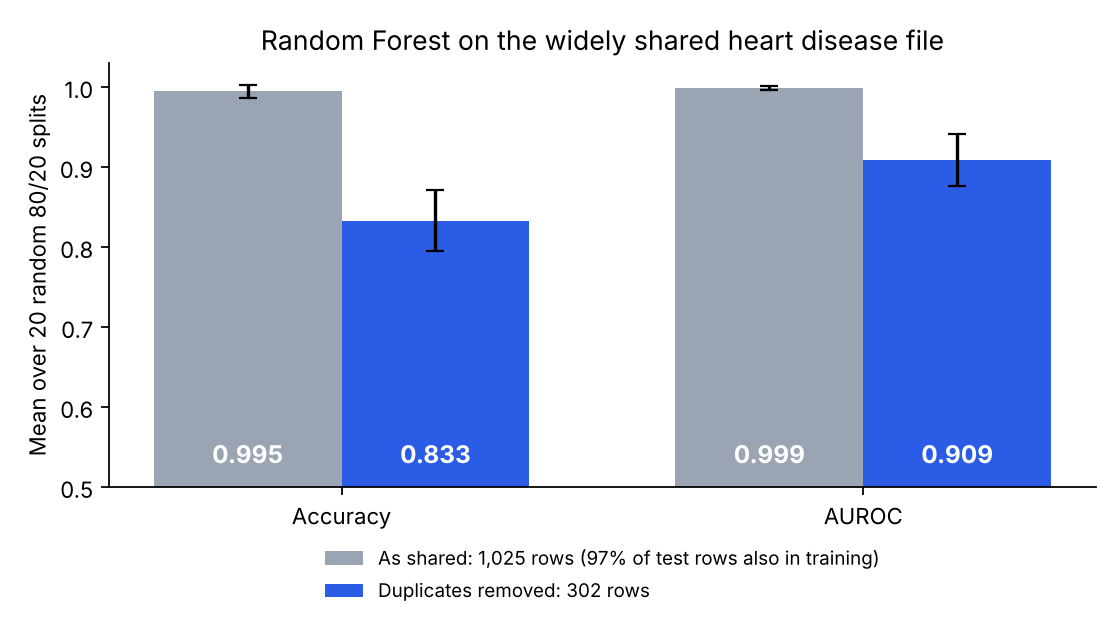
\includegraphics[width=0.72\linewidth]{figures/leakage.png}
\caption{Accuracy and AUROC with and without duplicate rows (error bars: one SD over 20 splits).}
\label{fig:leak}
\end{figure}

\subsection{Internally, simple and modern models are level}
Table~\ref{tab:cv} shows internal cross-validation. All six models fall between 0.882 and 0.907 AUROC, a range comparable to the fold-to-fold standard deviation (0.015--0.024). TabPFN is marginally best, and logistic regression is essentially level with it, while LightGBM is lowest and least well calibrated. This is consistent with the observation that flexible models rarely outperform logistic regression on small clinical tables \citep{christodoulou2019lr}.

\begin{table}[t]
\centering
\caption{Internal validation: repeated stratified 5-fold cross-validation (5 repeats), mean $\pm$ SD over 25 folds.}
\label{tab:cv}
\resizebox{\linewidth}{!}{\begin{tabular}{lcccccc}
\toprule
Model & AUROC & AUPRC & Brier & ECE & Sensitivity & Specificity \\
\midrule
TabPFN & 0.907 $\pm$ 0.018 & 0.912 $\pm$ 0.025 & 0.120 $\pm$ 0.013 & 0.062 $\pm$ 0.016 & 0.861 $\pm$ 0.031 & 0.797 $\pm$ 0.043 \\
Logistic regression & 0.904 $\pm$ 0.015 & 0.912 $\pm$ 0.023 & 0.122 $\pm$ 0.011 & 0.066 $\pm$ 0.016 & 0.850 $\pm$ 0.030 & 0.800 $\pm$ 0.041 \\
Random forest & 0.895 $\pm$ 0.023 & 0.898 $\pm$ 0.028 & 0.129 $\pm$ 0.013 & 0.073 $\pm$ 0.014 & 0.863 $\pm$ 0.031 & 0.788 $\pm$ 0.042 \\
CatBoost & 0.894 $\pm$ 0.024 & 0.892 $\pm$ 0.030 & 0.129 $\pm$ 0.017 & 0.075 $\pm$ 0.020 & 0.852 $\pm$ 0.033 & 0.788 $\pm$ 0.045 \\
XGBoost & 0.893 $\pm$ 0.020 & 0.893 $\pm$ 0.026 & 0.127 $\pm$ 0.015 & 0.070 $\pm$ 0.016 & 0.853 $\pm$ 0.033 & 0.795 $\pm$ 0.041 \\
LightGBM & 0.882 $\pm$ 0.022 & 0.880 $\pm$ 0.028 & 0.139 $\pm$ 0.018 & 0.097 $\pm$ 0.024 & 0.842 $\pm$ 0.037 & 0.787 $\pm$ 0.039 \\
\bottomrule
\end{tabular}
}
\end{table}

\subsection{Discrimination drops at an unseen hospital}
Table~\ref{tab:loso} and Figure~\ref{fig:loso} report LOHO results. Cleveland and Hungary transfer well (0.85--0.90), close to internal estimates. At VA Long Beach every model drops to 0.70--0.73, and the upper bounds of the intervals (0.79--0.82) lie below the internal estimates; mean specificity across models falls to 0.56. Switzerland shows similar point estimates, but with 115 of 123 patients diseased its estimate rests on 8 negatives, and intervals span roughly 0.47 to 0.97; we do not interpret it. No model is consistently better than logistic regression out of site.

\begin{table}[t]
\centering
\caption{Leave-one-hospital-out AUROC [95\% bootstrap CI], all 13 attributes.}
\label{tab:loso}
\resizebox{\linewidth}{!}{\begin{tabular}{lcccc}
\toprule
Model & Cleveland & Hungary & Switzerland & VA Long Beach \\
\midrule
Logistic regression & 0.891 [0.85, 0.93] & 0.904 [0.87, 0.94] & 0.718 [0.49, 0.94] & 0.717 [0.64, 0.80] \\
Random forest & 0.883 [0.84, 0.92] & 0.893 [0.85, 0.93] & 0.727 [0.50, 0.97] & 0.724 [0.64, 0.81] \\
TabPFN & 0.881 [0.84, 0.92] & 0.898 [0.86, 0.94] & 0.700 [0.47, 0.92] & 0.728 [0.65, 0.82] \\
XGBoost & 0.853 [0.81, 0.90] & 0.880 [0.84, 0.92] & 0.714 [0.48, 0.95] & 0.698 [0.61, 0.79] \\
LightGBM & 0.856 [0.81, 0.89] & 0.871 [0.83, 0.91] & 0.710 [0.48, 0.94] & 0.704 [0.61, 0.80] \\
CatBoost & 0.866 [0.82, 0.90] & 0.855 [0.81, 0.90] & 0.698 [0.48, 0.94] & 0.715 [0.63, 0.81] \\
\bottomrule
\end{tabular}
}
\end{table}

\begin{figure}[t]
\centering
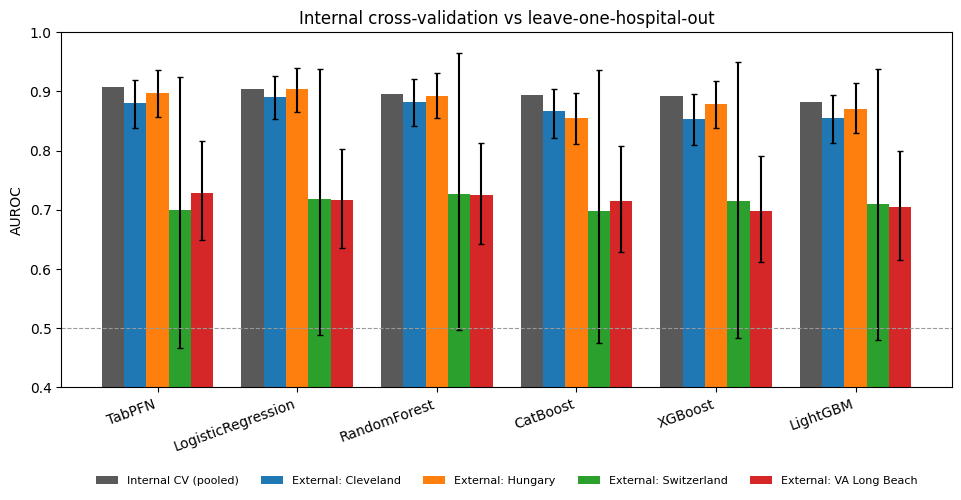
\includegraphics[width=0.95\linewidth]{figures/internal_vs_external.png}
\caption{Internal cross-validation AUROC against AUROC on each held-out hospital (error bars: 95\% bootstrap CI).}
\label{fig:loso}
\end{figure}

\subsection{Calibration does not transfer}
Internally, ECE was 0.06--0.10. Out of site, calibration follows the prevalence gap between training and test hospitals (Table~\ref{tab:cal}, Figure~\ref{fig:cal}). Models over-predict risk in Hungary (observed-to-expected 0.65--0.79) and under-predict in Switzerland (1.31--1.48) and at VA (1.05--1.23); intercepts at Switzerland are about $+2.4$ on the logit scale. Calibration slopes below 1 for most boosted models indicate predictions that are too extreme at new sites. Any deployment would require local recalibration.

\begin{table}[t]
\centering
\caption{Calibration on held-out hospitals (all attributes): observed-to-expected ratio / calibration intercept / calibration slope.}
\label{tab:cal}
\resizebox{\linewidth}{!}{\begin{tabular}{lcccc}
\toprule
Model & Cleveland & Hungary & Switzerland & VA Long Beach \\
\midrule
Logistic regression & 1.39 / +0.98 / 0.95 & 0.76 / -0.85 / 1.22 & 1.36 / +2.37 / 0.60 & 1.05 / +0.53 / 0.54 \\
Random forest & 0.80 / -1.08 / 2.06 & 0.65 / -1.44 / 1.78 & 1.46 / +2.37 / 1.11 & 1.22 / +0.82 / 0.69 \\
TabPFN & 0.80 / -0.90 / 1.33 & 0.66 / -1.42 / 1.34 & 1.40 / +2.43 / 0.53 & 1.11 / +0.64 / 0.56 \\
XGBoost & 0.84 / -0.55 / 0.91 & 0.76 / -0.82 / 0.91 & 1.46 / +2.56 / 0.68 & 1.23 / +0.93 / 0.37 \\
LightGBM & 0.87 / -0.39 / 0.58 & 0.79 / -0.74 / 0.56 & 1.31 / +2.37 / 0.46 & 1.14 / +0.80 / 0.30 \\
CatBoost & 1.01 / +0.03 / 0.86 & 0.76 / -0.77 / 0.76 & 1.48 / +2.61 / 0.52 & 1.12 / +0.77 / 0.40 \\
\bottomrule
\end{tabular}
}
\end{table}

\begin{figure}[t]
\centering
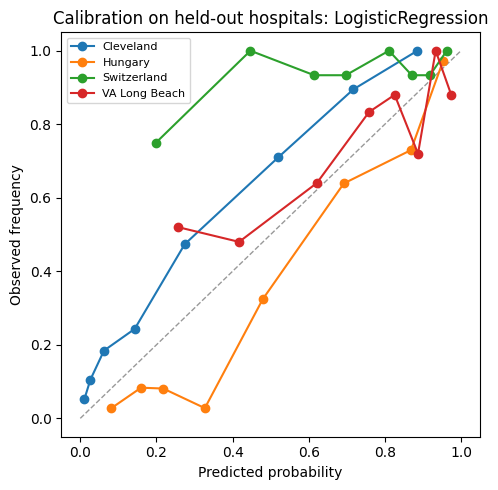
\includegraphics[width=0.5\linewidth]{figures/calibration_loso.png}
\caption{Reliability curves on each held-out hospital for logistic regression (quantile bins).}
\label{fig:cal}
\end{figure}

\subsection{Missingness indicators act as a site signal}
The most influential SHAP features for XGBoost are clinically plausible: asymptomatic chest pain, exercise-induced angina, ST depression, male sex, a flat ST slope and the number of vessels (Figure~\ref{fig:shap}). However, three of the 15 most influential inputs are missing-value indicators, for cholesterol, \texttt{ca} and fasting blood sugar. Because cholesterol is never recorded in Switzerland, where 93.5\% of patients have disease, its indicator is effectively a proxy for the hospital. This is a shortcut in the sense of \citet{geirhos2020shortcut}: it helps on pooled data but carries no physiological meaning and will not transfer to a site with different recording practice.

Excluding ST slope, \texttt{ca} and \texttt{thal} (Table~\ref{tab:core}) reduced AUROC at Cleveland, where these attributes are recorded (logistic regression 0.891 to 0.857), and increased it at Switzerland for all six models and at VA for five of six (for example random forest at Switzerland 0.727 to 0.789; TabPFN at VA 0.728 to 0.746). The intervals overlap, so this evidence is suggestive.

\begin{figure}[t]
\centering
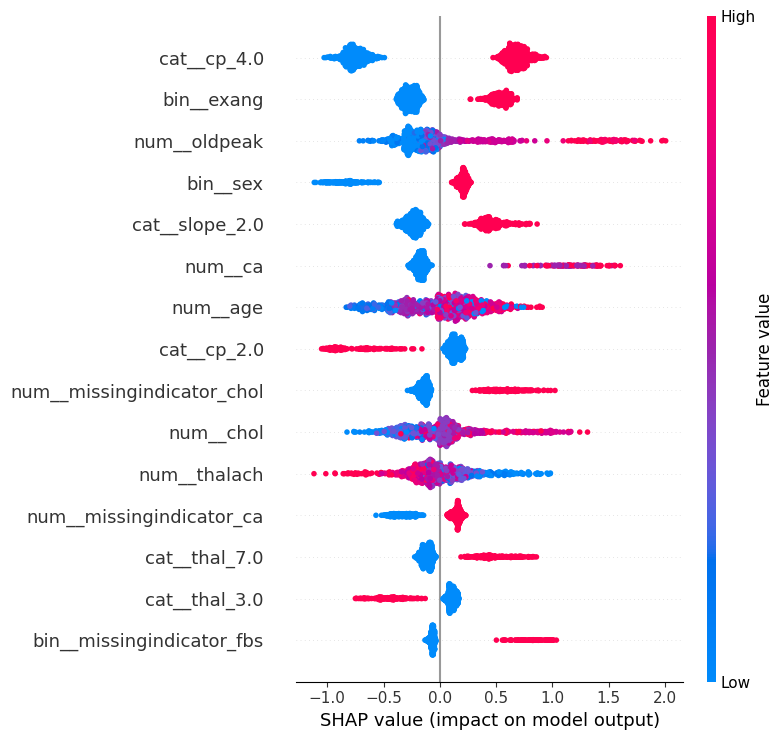
\includegraphics[width=0.62\linewidth]{figures/shap_summary.png}
\caption{SHAP summary for XGBoost trained on all 918 patients. Features prefixed \texttt{missingindicator} encode whether a value was recorded.}
\label{fig:shap}
\end{figure}

\begin{table}[t]
\centering
\caption{Leave-one-hospital-out AUROC [95\% CI] with the core feature set (without ST slope, \texttt{ca} and \texttt{thal}).}
\label{tab:core}
\resizebox{\linewidth}{!}{\begin{tabular}{lcccc}
\toprule
Model & Cleveland & Hungary & Switzerland & VA Long Beach \\
\midrule
Random forest & 0.865 [0.82, 0.90] & 0.869 [0.82, 0.91] & 0.789 [0.60, 0.98] & 0.730 [0.64, 0.82] \\
TabPFN & 0.864 [0.82, 0.90] & 0.876 [0.83, 0.92] & 0.746 [0.53, 0.96] & 0.746 [0.66, 0.83] \\
Logistic regression & 0.857 [0.82, 0.90] & 0.883 [0.84, 0.92] & 0.735 [0.51, 0.95] & 0.731 [0.64, 0.81] \\
XGBoost & 0.847 [0.80, 0.89] & 0.859 [0.81, 0.90] & 0.773 [0.57, 0.97] & 0.717 [0.63, 0.80] \\
LightGBM & 0.841 [0.80, 0.88] & 0.861 [0.82, 0.90] & 0.760 [0.56, 0.96] & 0.700 [0.62, 0.79] \\
CatBoost & 0.837 [0.79, 0.88] & 0.863 [0.82, 0.90] & 0.732 [0.50, 0.96] & 0.720 [0.63, 0.80] \\
\bottomrule
\end{tabular}
}
\end{table}

\subsection{Subgroups}
Using out-of-fold predictions of logistic regression, the model with the best mean LOHO AUROC, discrimination was similar for women and men and lowest in patients aged 60 and over (Table~\ref{tab:sub}), the group with the highest prevalence (73.1\%).

\begin{table}[t]
\centering
\caption{Subgroup AUROC of logistic regression (out-of-fold, internal cross-validation).}
\label{tab:sub}
\begin{tabular}{lrrc}
\toprule
Group & $n$ & Prevalence & AUROC [95\% CI] \\
\midrule
Women & 193 & 25.9\% & 0.916 [0.866, 0.955] \\
Men & 725 & 63.2\% & 0.882 [0.857, 0.907] \\
Age $<$ 50 & 291 & 38.1\% & 0.920 [0.885, 0.950] \\
Age 50--59 & 374 & 56.7\% & 0.898 [0.865, 0.931] \\
Age $\geq$ 60 & 253 & 73.1\% & 0.837 [0.774, 0.893] \\
\bottomrule
\end{tabular}

\end{table}

\section{Discussion}
Three practical lessons follow. First, any score reported on the 1,025-row merged file should be treated as unreliable unless duplicates were removed before splitting; near-perfect accuracies on that file are expected from memorisation alone. Second, on the clean four-hospital data a regularised logistic regression is as good as gradient boosting and a tabular foundation model internally, and no better or worse externally; claims of superiority for complex models on these data should be judged against this baseline and its variability. Third, internal cross-validation on pooled sites overstates performance at a new site, and probabilities are not portable across sites with different prevalence. Reporting guidance for clinical prediction models already asks for external validation and calibration \citep{collins2024tripodai}; our results show why both matter even for a benchmark this familiar.

The missingness finding generalises beyond this dataset. When data from several sources are pooled, which values are missing often depends on the source rather than on the patient. Missing-value indicators, a standard and often helpful imputation choice, then give the model a direct route to the source label, as hospital identity did for chest radiographs in \citet{zech2018variable}. Leave-one-source-out evaluation, explanation methods and feature ablations are simple ways to detect this.

\paragraph{Limitations.} The data were collected in the 1980s, the label is angiographic disease rather than a modern outcome, and the cohorts are small. Hyperparameters were not tuned; tuning could change the ranking of models slightly but is unlikely to remove the external drop. The Switzerland site is too small and imbalanced to evaluate, subgroup analysis used a single model, and SHAP values describe one model fitted on pooled data. Exact duplicates were removed but near-duplicates were not examined. We did not evaluate recalibration or site-adaptation methods, which are natural next steps.

\section{Conclusion}
On the UCI heart disease data, duplicate records explain near-perfect published scores, simple models match modern ones, performance drops and calibration breaks at an unseen hospital, and models partly learn the hospital through missing data. We recommend de-duplication before splitting, leave-one-hospital-out evaluation and calibration reporting as the minimum standard for future work on these data.

\section*{Data and code availability}
All code, tests, result tables and figures are available at \url{https://github.com/MHKhan50/heart-disease}. The complete analysis runs on a free Kaggle CPU session: \url{https://www.kaggle.com/code/muzammalhussain11/heart-disease-v2-leakage-audit-hospital-split}. The UCI data are available under a CC BY 4.0 licence \citep{uciheart}.

\bibliographystyle{plainnat}
\bibliography{refs}
\end{document}
